\documentclass[11pt]{amsart}
%%%%%%%%%%%%%% Packages
\usepackage{amssymb,amsfonts,amsthm,amsmath}
%%%%%% Better tables
\usepackage{tabu}
%%%%%%%%
\usepackage{subcaption}
\usepackage[english]{babel}
\usepackage[all,cmtip]{xy}
\usepackage{tikz}
\usepackage{mathtools}
\usepackage{tensor}
\usepackage{csquotes}
%\usepackage{stix}
\usetikzlibrary{arrows,chains,matrix,positioning,scopes}
%\usepackage{mathrsfs}
%\usepackage[notcite,notref]{showkeys}


%%%%%%%%%%% Tikz
\makeatletter
\tikzset{join/.code=\tikzset{after node path={%
\ifx\tikzchainprevious\pgfutil@empty\else(\tikzchainprevious)%
edge[every join]#1(\tikzchaincurrent)\fi}}}
\makeatother
\tikzset{>=stealth',every on chain/.append style={join},
         every join/.style={->}}

        

%%%%%%%%%%%% Personalized commands and environments

\newcommand{\inputc}[1]{ \raisebox{-0.5\height}{\input{#1}} }
\newtheorem{theorem}{Theorem}[section]
\newtheorem{lemma}[theorem]{Lemma}
\newtheorem{corollary}[theorem]{Corollary}
\newtheorem{definition}[theorem]{Definition}
\newtheorem{proposition}[theorem]{Proposition}
\newtheorem{remark}[theorem]{Remark}
\newtheorem{example}{Example}[section]
%\newtheorem{theorem*}{Theorem}

\newcommand{\func}[3]{{#1} : {#2} \longrightarrow {#3}}
\numberwithin{equation}{section}
\newcommand{\dbar}{\bar{\partial}}
\newenvironment{myproof}{\noindent{it Proof}
\setlength{\parindent}{0mm}}
{$\hfill \bs$}


%%%%%%%%%%%%%%%%%%%%%%%% Title and Author information

\title{MAT 203 Summer I 2020: Supplemental notes on polar coordinates}


\author[M. Gomes]{Marlon Gomes}
\address{Mathematics Department, Stony Brook University,
100 Nicolls Road, Math Tower, 
Stony Brook, NY, 11794, USA} \email{mgomes@math.stonybrook.edu}



%%%%%%%%%%% Text

\begin{document}

\begin{abstract}
In these notes we present an updated account of polar coordinates, which should be used for all questions involving this concept in this course. 
\end{abstract}

\maketitle

\section{Introduction}
The notion of polar coordinates, in particular graphs of polar equations has long caused confusion in Calculus students. In particular, the convention adopted by our textbook is in line with what is usually taught at a pre-Calculus level, but incompatible with that of Advanced Mathematics. As we aim to prepare students for courses up the ladder, here we seek to dismisfity these concepts through numerous examples of polar coordinate graphs. 

Recall that the polar coordinate system is characterized by two components:
\begin{itemize}
\item a radial component, denoted $r$, measuring the distance to the origin;
\item an angular component, denoted $\theta$, measuring the angle between the vector and the positive $x$-axis, measured in counter-clockwise sense.
\end{itemize}

There is an issue with uniqueness. Of course, pairs whose angular coordinates differ by multiples of $2\pi$, but radial coordinates are the same represent the same point in the plane. A coordinate system must be unambiguous, thus, we will set the convention that $\theta$ varies in the range $[0,2\pi)$. This addresses all ambiguities with respect to the angular coordinate other than the representation of the origin, which can take the form $(0,\theta)$ for any angle $\theta$. In addition, we leave little interpretation for $r$: it must be a non-negative number (by constrast, your textbook uses negative values of $r$). The relation between Cartesian and Polar coordinates is expressed by the equations below, 
\begin{align*}
x & = r\cos(\theta), \\
y & = r\sin(\theta),
\end{align*}
with $r$ and $\theta$ subject to the constraints discussed above. 

\section{Polar graphs}
In what follows we wish to describe how to graph curves defined by polar equations. In doing so, at times there will be polar equations for which the value of $r$ is negative. The convention we will adopt here is that no plot should be drawn in the angular regions where this occurs. By contrast, your textbook suggests that one should reverse the orientation, drawing a point with the same magnitude as $|r|$, but at a diametrically oposed angle. While this leads to pretty pictures, it makes for poor Calculus, as we will explain in the next section. 

\begin{example}
Consider the graph of the polar curve 
\begin{equation*}
r = 1.
\end{equation*}
This equation states is satisfied by all points whose distance to the origin is 1, that is, points lying along the circle of radius 1 about the origin. This is a simple enough example that no issues arise. Below is a plot of the corresponding curve. 
\begin{center}
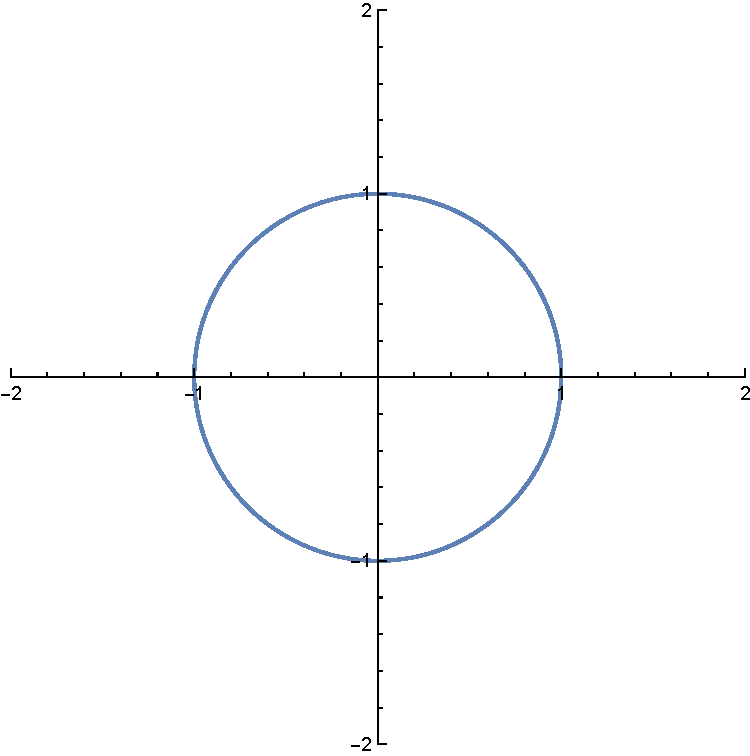
\includegraphics[scale=0.3]{polar_p1.pdf}
\end{center}
\end{example}

\begin{example}
Consider the cardiod given by the polar equation
\begin{equation*}
r = 2-2\sin(\theta).
\end{equation*}
To plot this curve, for each value of $\theta$ we mark a point along the ray of angle $\theta$ with the positive $x$-axis, situated at distance $r$ from the origin. The table below contains a few sample values of $(r,\theta)$. 
\begin{center}
{\tabulinesep=1.2mm
\begin{tabu}{|c|c|c|c|c|c|c|c|c|c|}
\hline 
$r$ & $0$ & $\frac{\pi}{4}$ & $\frac{\pi}{2}$ & $\frac{3\pi}{4}$ & $\pi$ & $\frac{5\pi}{4}$ & $\frac{3\pi}{2}$ & $\frac{7\pi}{4}$ & $2\pi$\\ 
\hline 
$\theta$ & $2$  & $2-\sqrt{2}$ & 0 & $2-\sqrt{2}$ & $2$ & $2+\sqrt{2}$ & $4$ & $2+\sqrt{2}$ & $2$\\ 
\hline 
\end{tabu} }
\end{center}

Below is a plot of the corresponding curve, with polar coordinate grids shown.
\begin{center}
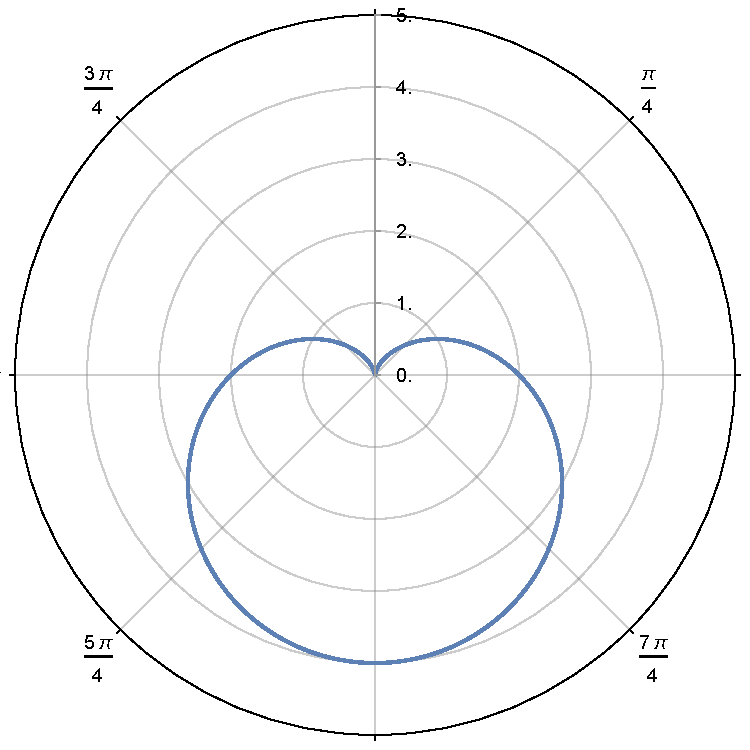
\includegraphics[scale=0.5]{polar_p2.pdf}
\end{center}
\end{example}

\begin{example}
The equation below describes a spiral, 
\begin{equation*}
r = \theta
\end{equation*}
Below is a plot of this polar curve, for $\theta \in [0,8\pi]$.
\begin{center}
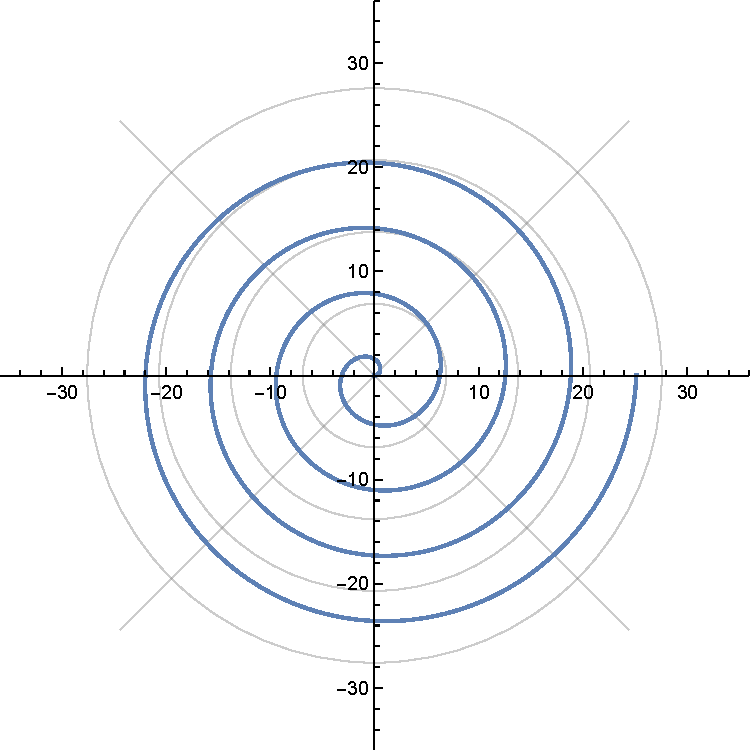
\includegraphics[scale=0.5]{polar_p3.pdf}
\end{center} 
\end{example}

\begin{example}
The case of the polar curve 
\begin{equation*}
r = sin(2\theta)
\end{equation*}
leads to conflict with our textbook's convention. This is due to the the fact that for angles
\begin{equation*}
\theta \in \left(\frac{\pi}{2},\pi\right) \cup \left(\frac{3\pi}{2},2\pi\right)
\end{equation*}
the corresponding value of $r$ would be negative. As such values are out of the range of acceptable values for $r$, according to our convention, we draw nothing on the polar chart. Meanwhile the authors of our textbook would draw points by reversing the orientation. Below is a comparative between the convention we adopt in this course, on the left, and the convention the textbook adopts, on the right. 

\begin{figure}
  \begin{subfigure}[b]{0.4\textwidth}
    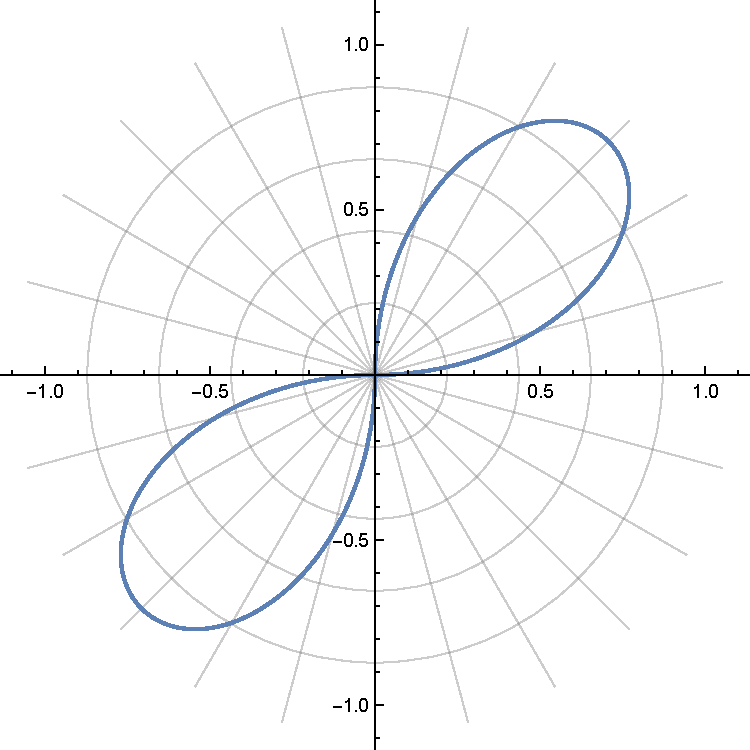
\includegraphics[width=\textwidth]{polar_p4.pdf}
    \caption{Our convention}
    \label{fig:1}
  \end{subfigure}
  \hfill
  \begin{subfigure}[b]{0.4\textwidth}
    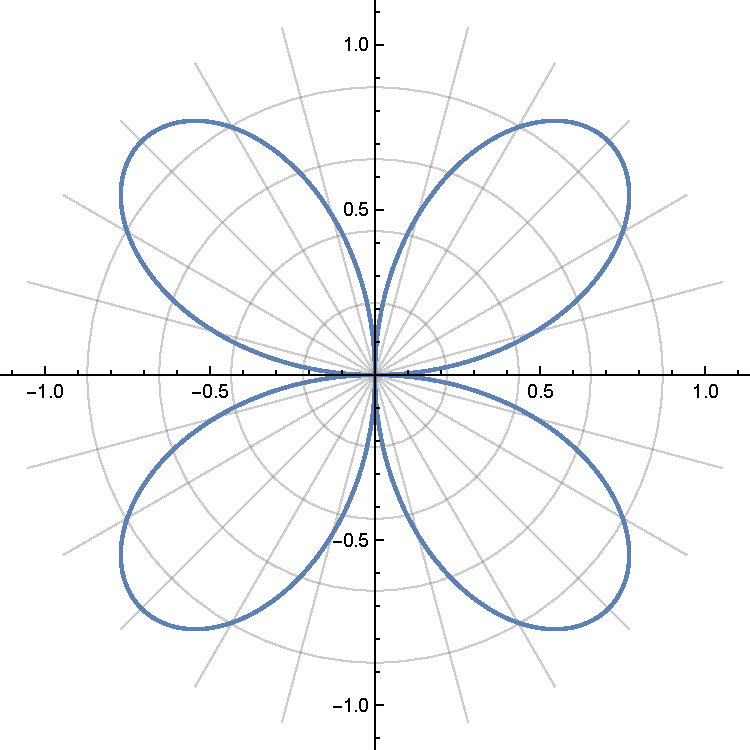
\includegraphics[width=\textwidth]{polar_p5.pdf}
    \caption{Textbook's convention}
    \label{fig:2}
  \end{subfigure}
  \hfill
\end{figure}
\end{example}

\begin{example}
Let's revisit example 2.4, the polar curve defined by the equation
\begin{equation*}
r=\sin(2\theta).
\end{equation*}
By means of double angle formulas, we find
\begin{equation*}
r=2\cos(\theta)\sin(\theta),
\end{equation*}
which when multiplied by $r^2$ (a bijective transformation when $r=\neq0$), we find the Cartesian equivalent
\begin{align*}
r^3 & = 2(r\cos(\theta))(r\sin(\theta)), \\
(x^2+y^2)^{\frac{3}{2}} & = 2xy.
\end{align*}
As the left-hand side is non-negative, one should only draw points in the first and third quadrants, where both coordinates have the same sign. Below is a computer-generated plot of the curve defined by the Cartesian equation above
\begin{center}
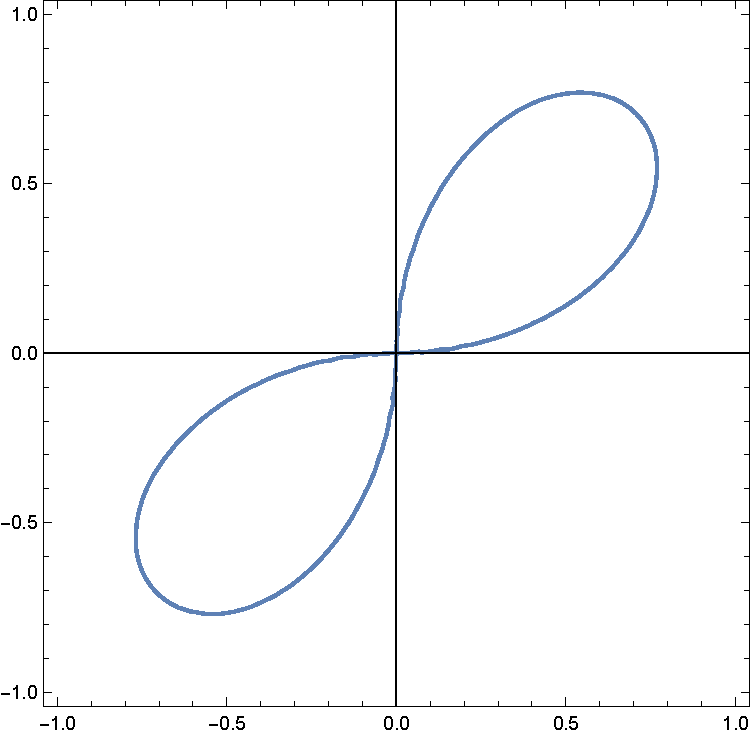
\includegraphics[scale=0.4]{polar_p6.pdf}
\end{center} 
If one wishes to obtain the four-petal rose as described by the textbook, there is an easy fix:
\begin{equation*}
r=|\sin(2\theta)|.
\end{equation*}
The corresponding cartesian equation is represented below. 
\begin{equation}
(x^2+y^2)^{\frac{3}{2}}  = 2|xy|,
\end{equation}
whose plot is 
\begin{center}
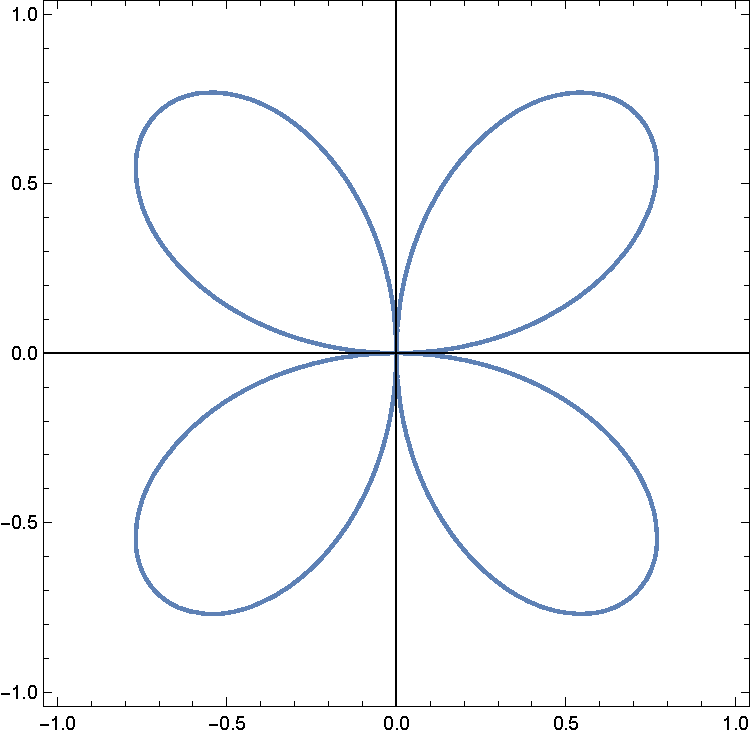
\includegraphics[scale=0.4]{polar_p7.pdf}
\end{center} 
This avoids the issues with double counting of areas and arclength the textbook refers to in page 730. 
\end{example}


\end{document}